\chapter{Results}
\label{ch:results}

All results in this chapter are computed on the full official 7{,}600-record AG News test set, from
each model's restored best-validation checkpoint. The test set was used once.

\section{Training dynamics}

\begin{table}[ht]
\centering
\caption{Training summary. Both models stopped early, well inside the epoch cap of eight.}
\label{tab:training_summary}
\begin{tabular}{lrr}
\toprule
\textbf{Quantity} & \textbf{BiLSTM} & \textbf{Transformer} \\
\midrule
Learning rate                      & $10^{-3}$ & $3\times10^{-4}$ \\
Epochs run                         & 3 & 5 \\
Best epoch                         & 1 & 3 \\
Best validation macro-$F_1$ & 0.9091 & 0.9077 \\
Total training time (s)            & 126 & 353 \\
\bottomrule
\end{tabular}
\end{table}

Figure~\ref{fig:curves} shows the learning curves. Two observations follow, and the first is
reported because it qualifies the comparison rather than because it flatters it.

\keypoint{Both models overfit rapidly, and the recurrent model peaked after a single epoch.}
Training loss continues to fall throughout, while validation loss rises from epoch~2 onward in both
cases. The early-stopping criterion detected this and restored the correct checkpoint, but the
consequence is that the recurrent model's \emph{effective} training budget was one epoch of 422
optimisation steps. The epoch cap of eight was never the binding constraint for either model.

\keypoint{The Transformer converges more slowly but more smoothly.} It reaches its optimum at epoch
3 rather than epoch 1, consistent with its lower learning rate, and its validation macro-$F_1$
curve is less abrupt. Neither model benefits from further training under this configuration.

\begin{figure}[ht]
\centering
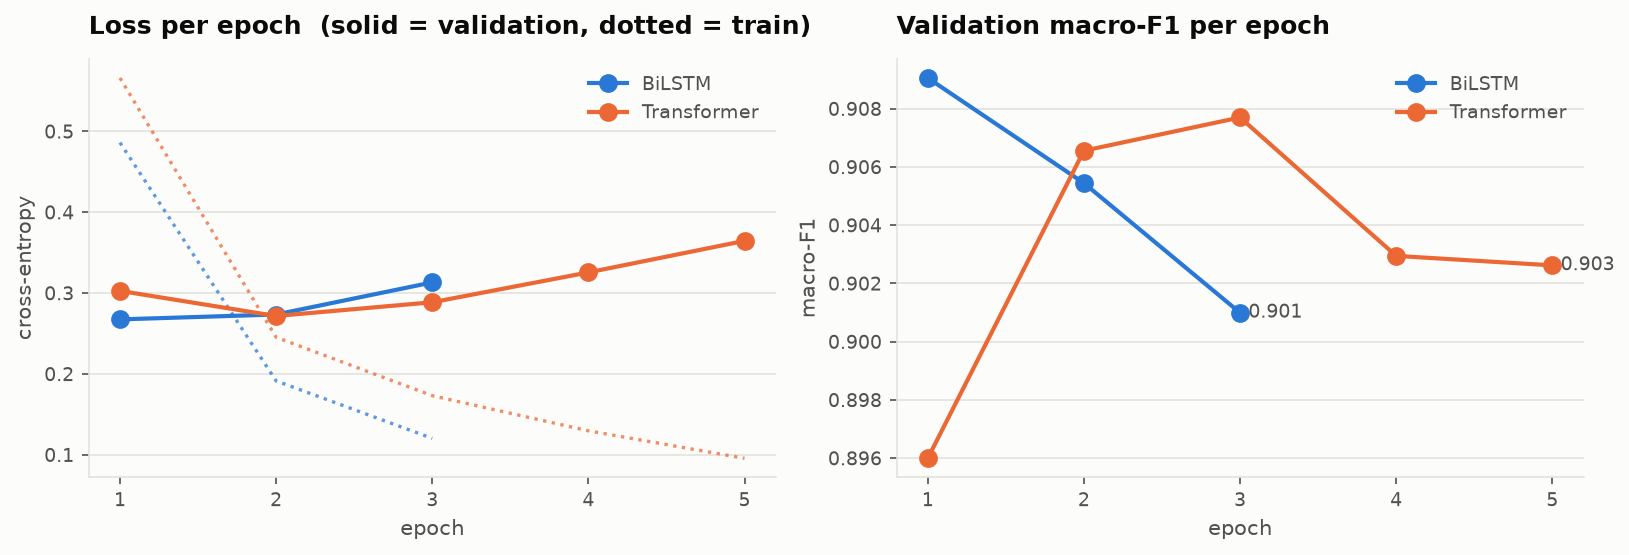
\includegraphics[width=\textwidth]{figures/fig3_learning_curves.png}
\caption[Learning curves]{Learning curves. Left: cross-entropy per epoch, solid for validation and
dotted for training. Right: validation macro-$F_1$. The divergence between training
and validation loss from epoch~2 is the overfitting referred to in the text.}
\label{fig:curves}
\end{figure}

\section{Headline results}

\begin{table}[ht]
\centering
\caption[Headline test-set results]{Headline results on the held-out test set. The accuracy
difference is 0.09 percentage points, corresponding to seven documents out of 7{,}600.}
\label{tab:headline}
\begin{tabular}{lrrrr}
\toprule
\textbf{Model} & \textbf{Accuracy} & \textbf{Macro $F_1$} & \textbf{Weighted $F_1$} & \textbf{Test loss} \\
\midrule
BiLSTM      & 0.9114 & 0.9111 & 0.9111 & 0.2797 \\
Transformer & 0.9105 & 0.9104 & 0.9104 & 0.2944 \\
\midrule
Difference  & 0.0009 & 0.0007 & 0.0007 & $-0.0147$ \\
\bottomrule
\end{tabular}
\end{table}

Both models land in the 90--92\% band anticipated by the survey of published results in
Table~\ref{tab:prior}, which is the expected range for a from-scratch model without pretraining.
The recurrent model is nominally ahead on every metric except test loss.

\keypoint{This difference must not be interpreted before it is tested.} A gap of 0.09 percentage
points on 7{,}600 documents is seven documents. Section~\ref{sec:significance} determines whether
that is distinguishable from noise. It is not.

\section{Per-class performance}

\begin{table}[ht]
\centering
\caption[Per-class results]{Per-class precision, recall and $F_1$. Support is 1{,}900
documents for every class.}
\label{tab:per_class}
\begin{tabular}{lrrrcrrr}
\toprule
 & \multicolumn{3}{c}{\textbf{BiLSTM}} & & \multicolumn{3}{c}{\textbf{Transformer}} \\
\textbf{Class} & \textbf{P} & \textbf{R} & \textbf{$F_1$} & & \textbf{P} & \textbf{R} & \textbf{$F_1$} \\
\midrule
World     & 0.9366 & 0.8789 & 0.9069 & & 0.9227 & 0.9053 & 0.9139 \\
Sports    & 0.9459 & 0.9853 & 0.9652 & & 0.9553 & 0.9674 & 0.9613 \\
Business  & 0.8850 & 0.8705 & 0.8777 & & 0.8889 & 0.8674 & 0.8780 \\
Sci/Tech  & 0.8791 & 0.9111 & 0.8948 & & 0.8754 & 0.9021 & 0.8885 \\
\midrule
Macro avg & 0.9117 & 0.9114 & 0.9111 & & 0.9106 & 0.9105 & 0.9104 \\
\bottomrule
\end{tabular}
\end{table}

\begin{figure}[ht]
\centering
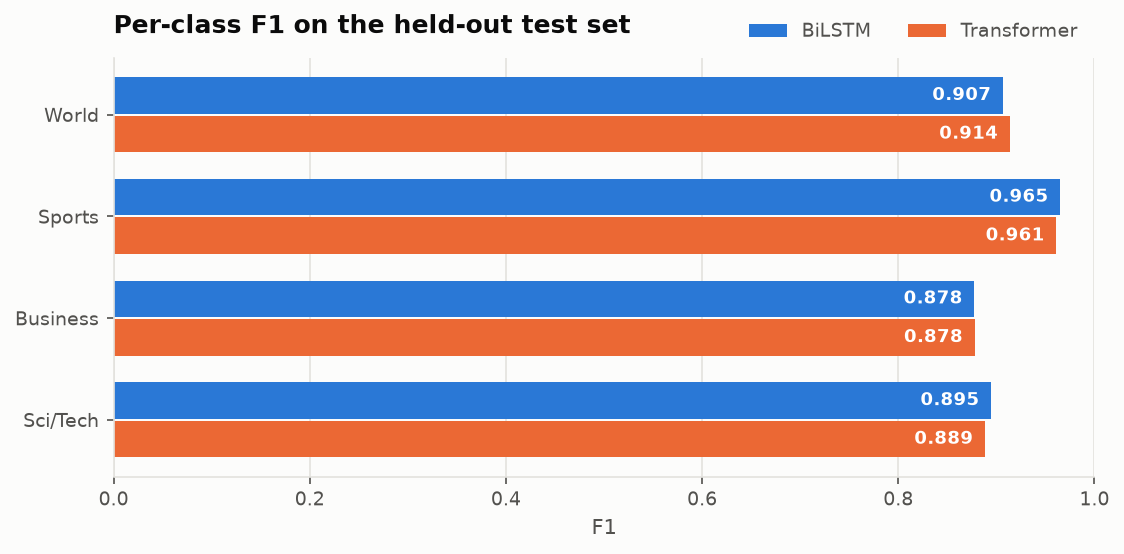
\includegraphics[width=\textwidth]{figures/fig1_per_class_f1.png}
\caption[Per-class F1 comparison]{Per-class $F_1$ for both models. The difficulty
ordering is identical: Sports is easiest for both, Business hardest for both.}
\label{fig:perclass}
\end{figure}

The striking feature of Table~\ref{tab:per_class} is not the magnitude of any difference but the
\emph{similarity of the profile}. Both models order the classes identically by difficulty:

\begin{center}
Sports ($\approx 0.96$) $\;>\;$ World ($\approx 0.91$) $\;>\;$ Sci/Tech ($\approx 0.89$) $\;>\;$ Business ($\approx 0.878$)
\end{center}

On Business the two models agree to four decimal places (0.8777 versus 0.8780). The two
architectures do not merely achieve the same aggregate accuracy; they find the same classes easy
and the same classes hard, to a degree that suggests both are limited by the same property of the
data rather than by their own representational capacity.

\section{Confusion structure}

\begin{figure}[ht]
\centering
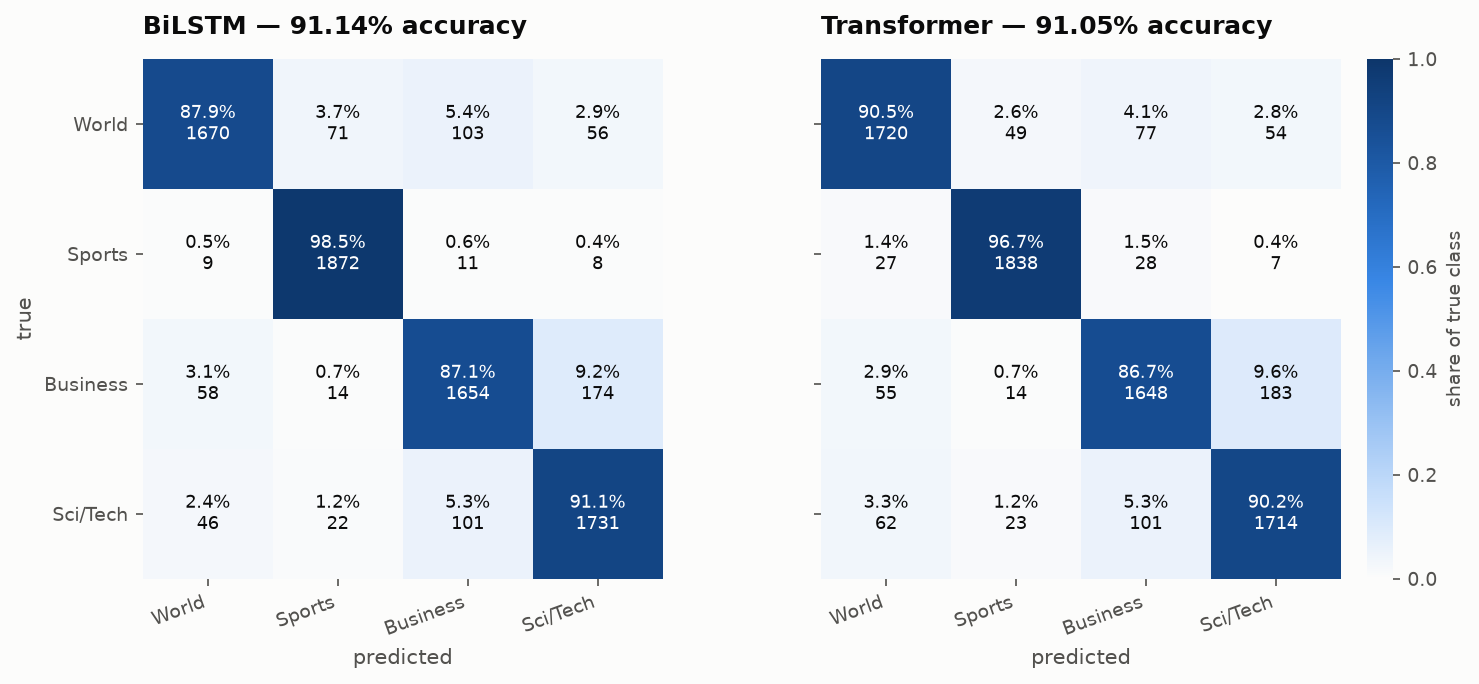
\includegraphics[width=\textwidth]{figures/fig2_confusion_matrices.png}
\caption[Confusion matrices]{Row-normalised confusion matrices on a shared colour scale. Each row
sums to 100\% of the true class. The dominant off-diagonal cell is Business predicted as Sci/Tech
for both models.}
\label{fig:confusion}
\end{figure}

\begin{table}[ht]
\centering
\caption{Largest off-diagonal confusions, as a proportion of the true class.}
\label{tab:confusions}
\begin{tabular}{llrr}
\toprule
\textbf{True} & \textbf{Predicted} & \textbf{BiLSTM} & \textbf{Transformer} \\
\midrule
Business & Sci/Tech & 9.2\% (174) & 9.6\% (183) \\
World    & Business & 5.4\% (103) & 4.1\% (77) \\
Sci/Tech & Business & 5.3\% (101) & 5.3\% (101) \\
World    & Sports   & 3.7\% (71)  & 2.6\% (49) \\
\bottomrule
\end{tabular}
\end{table}

The structure is consistent across both models. The dominant error is Business misclassified as
Sci/Tech, and its converse is the third largest. Together, the Business--Sci/Tech boundary accounts
for roughly a quarter of all errors made by either model.

Sports is nearly separable from everything else --- 98.5\% and 96.7\% recall --- which is
unsurprising given its highly distinctive vocabulary. The difficulty is concentrated entirely in
the commercial and technological categories, whose vocabularies overlap substantially.

\section{Statistical significance}
\label{sec:significance}

Applying McNemar's test as specified in Section~\ref{sec:mcnemar} to the paired predictions:

\begin{table}[ht]
\centering
\caption[McNemar contingency table]{McNemar contingency table on the 7{,}600 test documents.}
\label{tab:mcnemar}
\begin{tabular}{lrr}
\toprule
 & \textbf{BiLSTM correct} & \textbf{BiLSTM wrong} \\
\midrule
\textbf{Transformer correct} & 6{,}740 & 180 \\
\textbf{Transformer wrong}   & 187     & 493 \\
\bottomrule
\end{tabular}
\end{table}

The models agree on $6{,}740 + 493 = 7{,}233$ documents, or \textbf{94.78\%} of the test set. The
discordant set contains 367 documents: 187 answered correctly only by the recurrent model and 180
only by the Transformer.

Under the null hypothesis of equal error rates, the number falling to either model follows
$\operatorname{Binomial}(367, 0.5)$. The exact binomial test gives
\begin{equation}
p = 0.754 .
\end{equation}

\keypoint{The difference is not statistically significant at $\alpha = 0.05$.} A split of 187
against 180 is as close to an even division as a test set of this size can resolve. The correct
conclusion is that \textbf{the two architectures are indistinguishable in accuracy on this task} --
not that the recurrent model is marginally superior.

This is the central result of the study, and it would have been inaccessible from the headline
accuracy figures alone. A 0.09 percentage point gap presented without a significance test invites
exactly the over-interpretation that the test forecloses.

\section{Computational cost}
\label{sec:cost}

\begin{table}[ht]
\centering
\caption[Computational cost]{Computational cost on the CPU-only environment of
Table~\ref{tab:environment}.}
\label{tab:cost}
\begin{tabular}{lrr}
\toprule
\textbf{Measure} & \textbf{BiLSTM} & \textbf{Transformer} \\
\midrule
Non-embedding parameters  & 265{,}220 & 265{,}732 \\
Seconds per epoch         & 41.2 & 68.6 \\
Total training time (s)   & 126  & 353 \\
Inference (ms per 1{,}000 documents) & 138 & 335 \\
Test accuracy             & 0.9114 & 0.9105 \\
\bottomrule
\end{tabular}
\end{table}

At matched capacity and matched accuracy, the recurrent model trains \textbf{1.67 times faster per
epoch} and performs inference \textbf{2.43 times faster}.

\keypoint{This is the opposite of the expected result, and it requires careful interpretation
rather than explanation away.}

The standard argument, formalised in Table~\ref{tab:complexity}, is that recurrence requires $O(n)$
strictly sequential steps whereas self-attention requires $O(1)$, so attention should be faster in
wall-clock terms. That argument is correct, but it is an argument about \emph{parallelisability},
and it is conditional on two things that do not hold here.

First, \textbf{parallel hardware}. The advantage of $O(1)$ sequential depth is realised only when
there are parallel resources to exploit. On six CPU threads there is very little parallelism
available, so the Transformer cannot convert its structural advantage into elapsed time.

Second, \textbf{the relationship between $n$ and $d$}. Per-layer arithmetic is $O(n d^2)$ for
recurrence and $O(n^2 d)$ for self-attention. Self-attention performs less total arithmetic only
when $n < d$. Here $n = 64$ and $d = 128$, so the two are of the same order and neither dominates.
The Transformer performs more total floating-point work per document --- two encoder blocks of
four-head attention over all 64 positions, each with a 256-wide feed-forward sublayer --- while the
recurrent model performs less work spread over 64 sequential dispatches.

When neither parallelism nor arithmetic favours attention, the constant factors decide, and here
they favour recurrence.

\keypoint{What this result does and does not license.} It does not license the claim that recurrent
networks are faster than Transformers. It licenses the narrower and more useful claim that
\emph{at short sequence lengths on sequential hardware, the Transformer's architectural advantage
does not materialise in wall-clock terms}. The recurrent model's disadvantage grows linearly with
sequence length, and on parallel hardware the ordering would be expected to reverse. This is a
finding about regime, not about architecture, and it is actionable precisely for that reason.

\section{Qualitative error analysis}

\subsection{Documents both models misclassify}

Of the 7{,}600 test documents, 493 are misclassified by both models. Table~\ref{tab:both_wrong}
gives a representative sample.

\begin{table}[ht]
\centering
\caption[Documents misclassified by both models]{Representative documents misclassified by both
models. In each case the predicted label is defensible.}
\label{tab:both_wrong}
\begin{tabular}{llp{7.3cm}}
\toprule
\textbf{True} & \textbf{Both predicted} & \textbf{Document (truncated)} \\
\midrule
Sci/Tech & World    & U.N. Urges Funds to Curb African Locusts --- with swarms threatening crops in a number of African countries \ldots \\
World    & Sports   & Argentina Basketball Coach Magnano Quits --- Ruben Magnano, who coached Argentina to the Olympic gold medal \ldots \\
Business & Sci/Tech & SBC links e-mail, voice messages, fax --- SBC announced a new service that integrates voice messages, faxes \ldots \\
Business & World    & Nepal blockade `blow to tourism' --- Nepal tour operators say tourists cancelled millions of dollars of bookings \ldots \\
Sci/Tech & World    & Singapore Telecom ties up with Malaysia's TIME dotcom --- SingTel said it has \ldots \\
\bottomrule
\end{tabular}
\end{table}

In every case the prediction is defensible. A story about United Nations funding to control locust
swarms is an international affairs story \emph{and} an agricultural science story. A telecoms
merger is a business story \emph{and} a technology story. These are not model failures in any
useful sense; they are documents whose single gold label is one of several admissible choices.

This is the practical upper bound on achievable accuracy for the task, and it explains why the
published results in Table~\ref{tab:prior} compress into such a narrow band.

\subsection{Documents on which the models disagree}

\begin{table}[ht]
\centering
\caption[Documents on which the models disagree]{Documents where the two models differ. Several
turn on a single lexical cue.}
\label{tab:disagree}
\begin{tabular}{lllp{5.4cm}}
\toprule
\textbf{True} & \textbf{BiLSTM} & \textbf{Transf.} & \textbf{Document (truncated)} \\
\midrule
Sports   & Sports   & Business & Cape Town F1 bid --- plan to build a multi-million-dollar race track \ldots \\
World    & Business & World    & ConocoPhillips boosts LUKoil stake to 10 percent \ldots \\
Business & Sports   & Business & Banks seek court ruling over F1 --- three banks go to the High Court in London \ldots \\
Sports   & Sports   & World    & New Namath Book Is Fact, Not Fiction --- if you read the recent excerpt in Sports Illustrated \ldots \\
World    & World    & Business & Australia: Wallets trump war --- a majority oppose the Iraq war, but were more concerned \ldots \\
\bottomrule
\end{tabular}
\end{table}

The disagreements are instructive. Several documents contain strong lexical evidence for two
classes simultaneously --- \emph{Formula One} alongside \emph{multi-million-dollar}, or
\emph{banks} and \emph{High Court} alongside \emph{F1} --- and the two models resolve the conflict
differently. Notably, neither model is systematically correct in these cases: the first and third
examples show the models trading places on the same underlying ambiguity.

This is consistent with the statistical finding of Section~\ref{sec:significance}. The disagreements
are not evidence of a systematic difference in capability; they are what one would expect from two
comparably-capable models resolving genuinely ambiguous cases with different random tie-breaking.
